\documentclass{pnastwo}
\usepackage{pnastwoF}
\usepackage[numbers,round]{natbib}
\usepackage{graphicx}
\usepackage{amssymb,amsfonts,amsmath}
\usepackage[american]{babel}
\usepackage{color}

\newcommand{\red}[1]{\textcolor{red}{#1}}


%% OPTIONAL MACRO DEFINITIONS
\def\s{\sigma}

% Fix wierd behavior which prevents table captions from appearing for
% tables in the body of the article
\makeatletter
\long\def\@makecaption#1#2{%
\ifx\@captype

\let\currtabcaption\relax
\gdef\currtabcaption{
\tabnumfont\relax #1. \tabtextfont\relax#2\par
\vskip\belowcaptionskip 
}
\else
 \vskip\abovecaptionskip
  \sbox\@tempboxa{\fignumfont#1.\figtextfont\hskip.5em\relax #2}%
  \ifdim \wd\@tempboxa >\hsize
\fignumfont\relax #1.\figtextfont\hskip.5em\relax#2\par
  \else
    \global \@minipagefalse
    \hb@xt@\hsize{\hfil\box\@tempboxa\hfil}%
  \fi
\fi
}
\makeatother

% And another fix.  PNAS class loses the label of floats unless they       
% were defined with the [h] option (so not really floats at all).  It      
% all comes down to wrong scope in the following routine which pushes      
% out the floats onto the page.  This is the fixed version:        
\makeatletter                                  
\def\DonormalEndcol{%                              
%% top float ==>                               
\ifx\toporbotfloat\xtopfloat%                          
%% figure ==>                                  
  \ifcaptypefig%                               
  \expandafter\gdef\csname topfloat\the\figandtabnumber\endcsname{%    
  \vbox{\vskip\PushOneColTopFig%                       
  \unvbox\csname figandtabbox\the\loopnum\endcsname%               
  \vskip\abovefigcaptionskip%                          
  \csname caption\the\loopnum\endcsname%                   
  \csname letteredcaption\the\loopnum\endcsname%               
  \csname continuedcaption\the\loopnum\endcsname%              
  \csname letteredcontcaption\the\loopnum\endcsname            
  \ifredefining%                               
  \csname label\the\loopnum\endcsname%                     
  \expandafter\gdef\csname topfloat\the\loopnum\endcsname{}\fi}%       
  \vskip\intextfloatskip%%                         
  \vskip-4pt %% probably an artifact of topskip??              
}%                                     
\else%                                     
%% plate ==>                                   
  \ifcaptypeplate%                             
  \expandafter\gdef\csname topfloat\the\figandtabnumber\endcsname{%    
  \vbox{\vskip\PushOneColTopFig%                       
  \unvbox\csname figandtabbox\the\loopnum\endcsname            
  \vskip\abovefigcaptionskip                           
  \csname caption\the\loopnum\endcsname                    
  \csname letteredcaption\the\loopnum\endcsname                
  \csname continuedcaption\the\loopnum\endcsname               
  \csname letteredcontcaption\the\loopnum\endcsname            
  \ifredefining                                
  \csname label\the\loopnum\endcsname                      
  \expandafter\gdef\csname topfloat\the\loopnum\endcsname{}\fi}        
  \vskip\intextfloatskip %%                            
  \vskip-4pt %% probably an artifact of topskip??              
}%                                     
\else% table ==>                               
 \expandafter\gdef\csname topfloat\the\figandtabnumber\endcsname{%     
 \vbox{\vskip\PushOneColTopTab %%                      
 \csname caption\the\loopnum\endcsname                     
  \csname letteredcaption\the\loopnum\endcsname                
  \csname continuedcaption\the\loopnum\endcsname               
  \csname letteredcontcaption\the\loopnum\endcsname            
  \vskip\captionskip                               
  \unvbox\csname figandtabbox\the\loopnum\endcsname            
\ifredefining                                  
\csname label\the\loopnum\endcsname                    
\expandafter\gdef\csname topfloat\the\loopnum\endcsname{}\fi           
}\vskip\intextfloatskip %% why don't we need this?             
\vskip-10pt}                                   
\fi\fi%                                    
%                                      
\else% bottom float                            
%                                      
\ifcaptypefig                                  
\expandafter\gdef\csname botfloat\the\figandtabnumber\endcsname{%      
\vskip\intextfloatskip                             
\vbox{\unvbox\csname figandtabbox\the\loopnum\endcsname            
\vskip\abovefigcaptionskip                         
  \csname caption\the\loopnum\endcsname                    
  \csname letteredcaption\the\loopnum\endcsname%               
  \csname continuedcaption\the\loopnum\endcsname%              
  \csname letteredcontcaption\the\loopnum\endcsname%               
\vskip\PushOneColBotFig%%                          
\ifredefining%                                 
\csname label\the\loopnum\endcsname                    
\expandafter\gdef\csname botfloat\the\loopnum\endcsname{}\fi}}%        
\else                                      
\ifcaptypeplate                                
\expandafter\gdef\csname botfloat\the\figandtabnumber\endcsname{%      
\vskip\intextfloatskip                             
\vbox{\unvbox\csname figandtabbox\the\loopnum\endcsname            
\vskip\abovefigcaptionskip                         
  \csname caption\the\loopnum\endcsname                    
  \csname letteredcaption\the\loopnum\endcsname%               
  \csname continuedcaption\the\loopnum\endcsname%              
  \csname letteredcontcaption\the\loopnum\endcsname%               
\vskip\PushOneColBotFig%%                          
\ifredefining%                                 
\csname label\the\loopnum\endcsname                    
\expandafter\gdef\csname botfloat\the\loopnum\endcsname{}\fi}}%        
  \else% TABLE                                 
\expandafter\gdef\csname botfloat\the\figandtabnumber\endcsname{%      
  \vskip\intextfloatskip                           
\vbox{\csname caption\the\loopnum\endcsname                
  \csname letteredcaption\the\loopnum\endcsname                
  \csname continuedcaption\the\loopnum\endcsname               
  \csname letteredcontcaption\the\loopnum\endcsname%               
  \vskip.5\intextfloatskip                         
  \unvbox\csname figandtabbox\the\loopnum\endcsname%               
\vskip\PushOneColBotTab                            
\ifredefining%                                 
\csname label\the\loopnum\endcsname                    
\expandafter\gdef\csname botfloat\the\loopnum\endcsname{}\fi}}%        
\fi\fi\fi}                                 
\makeatother                                   

%%%%%%%%%%%%
%% For PNAS Only:
\url{www.pnas.org/cgi/doi/10.1073/pnas.xxxxxxxxxx}
\copyrightyear{2008}
\issuedate{Issue Date}
\volume{Volume}
\issuenumber{Issue Number}
%\setcounter{page}{2687} %Set page number here if desired
%%%%%%%%%%%%

% \authornote{Please address correspondence to: 

% \vspace{12 pt}
% Daniel Yurovsky

% Jordan Hall (Building 420)

% Stanford University

% 450 Serra Mall

% Stanford, CA 94305

% \vspace{12 pt}
% Email: yurovsky@stanford.edu 

% \vspace{12 pt}
% Word Count: 1999

% References: 40}

\begin{document}

\widowpenalty10000
\clubpenalty10000

\title{Developmental changes in the speed of social attention in early word Learning}
\author{Daniel Yurovsky\affil{1}{Department of Psychology, Stanford University}, Anna Wade\affil{2}{School of Medicine, University of California, San Francisco}, Allison M Kraus\affil{1}{}, Grace W. Gengoux\affil{3}{School of Medicine, Stanford University}, Antonio Hardan\affil{3}{}, \and Michael C. Frank\affil{1}{} }
\contributor{Submitted to Proceedings of the National Academy of Sciences
of the United States of America}

% \affiliation{Department of Psychology, Stanford University}
% \shorttitle{Synthesizing Cross-Situational Learning}
% \leftheader{Yurovsky \& Frank}

% \abstract{}

\maketitle

\begin{article}
\begin{abstract}
To begin learning the meaning of a word, a child must determine if this word is being used to refer to something in the immediate physical context. Social cues---like the eye-gaze of a helpful speaker---are powerful information sources for resolving this problem. Studies of children's gaze following have generally been concerned with its developmental origins, demonstrating measurable success in early infancy. We show that this ability has a long developmental trajectory, however: Slow, continuous improvements in speed of social information processing occur over the course of the first five years of life. This developing ability is a significant bottleneck on early word learning, predicting changes in children's learning of new words over the same time period. Finally, we show that the same bottleneck exists in children diagnosed with autism spectrum disorder. These results describe a route by which increases in social expertise can lead to changes in language learning ability and highlight the dependence of developmental outcomes on not just the existence of particular competencies, but on their proficient use in complex contexts.
\end{abstract}
\keywords{ language acquisition | word learning | social cues | cognitive development}

\subsection{Significance Statement}
The study of language development has historically focused on pinpointing children's earliest points of competence in each domain. Learning outside the laboratory is ultimately controlled by proficient use of these same mechanisms, however. While infants can follow social cues like eye-gaze early in their first year, we show that the speed and fidelity of this process improves continuously over the first five years of life. The problem of tracking social information is far from resolved for young infants; it remains a bottleneck on word learning for typically developing children into the preschool years and and does so for autistic children as well. This work highlights the importance of studying not just origins but also the developmental trajectories of higher-level cognitive processes.

\vspace{12 pt}

\dropcap{C}hildren's first five years are a time of rapid developmental change. One striking development is children's growing mastery of their native language. The typical child will go from saying her first word shortly before her first birthday to producing complex, grammatical sentences only a few years later. Perhaps because of the fundamentally discrete nature of the units of language itself, much work in language acquisition has focused specifically on the origins of these important abilities \cite[but c.f.][]{fernald1998, port2005}. Reviews of language development are generally a list of milestones: e.g., infants acquire the ability to use sequential statistics to segment speech at 8 months \cite{saffran1996}, begin to use co-occurrence statistics to learn word-object mappings at 12 months \cite{smith2008}, and begin to use syntax to infer the meanings around 24 months \cite{gertner2006}. New exciting work then is often a demonstration of some competence earlier than previously observed \cite{bergelson2012}. This research strategy stands in contrast to work in domains like visual and motor development, in which researchers have sought to measure continuous changes in children's abilities as they develop \cite{sokol1978, banks1980, forssberg1991, thelen1995}.

Here we take as a case study children's use of social information to infer the meanings of new words. Over the first five years, children acquire a productive vocabulary of approximately 4000--5000 words \cite{goulden1990}. Though these words belong to many grammatical categories, a large proportion are concrete nouns \cite{bates1994}. While acquiring a fully adult-like meaning for any of these nouns likely unfolds over multiple encounters, the very first problem a child faces when hearing a new word is referential uncertainty: Does the word refer to something in the current situation, and if so, what \cite{carey1978, yu2007, frank2009}? A powerful source of information for resolving this uncertainty is available in the social cues provided by the speaker: e.g., where is the speaker looking? Consequently, a large body of research has accumulated documenting young infants' abilities to track a speaker's social cues and use them to infer the target of her reference \cite[e.g.][]{scaife1975, baldwin1993, hollich2000, senju2008}.

This research has focused almost exclusively on discovering the earliest point of infants' competence in using social information. Underlying this focus is an implicit assumption that, once the general ability to use social cues is demonstrated, children's proficiency with processing these cues is relatively high \cite[e.g.][]{corkum1998, brooks2005, csibra2009}. Contradicting this assumption, however, some work has argued that rapid gaze-following may occur relatively rarely in natural interactions and may be difficult even for older children and adults under some circumstances \cite{loomis2008, vida2012, yu2013}. 
% Because higher-level cognitive processes like social inference and word learning must sit on top of lower-level cognitive architectures that change continuously over development, they must themselves show significant change beyond their early origins.

There are more basic reasons to assume that children's use of social information in word learning would have a protracted developmental trajectory, as well. Using social information to resolve referential uncertainty is a highly time-sensitive process of continuous re-allocation of attention between the speaker and the objects in the context. To learn from a given situation, learners must rapidly process the auditory and visual information they are receiving. Consequently, competence is not enough: the referential uncertainty problem should remain a problem in proportion to a child's developing ability to control her attention, process auditory and visual information, and hold the information in memory \cite{dempster1981, kail1991, gathercole2004}. 

\begin{figure*}
        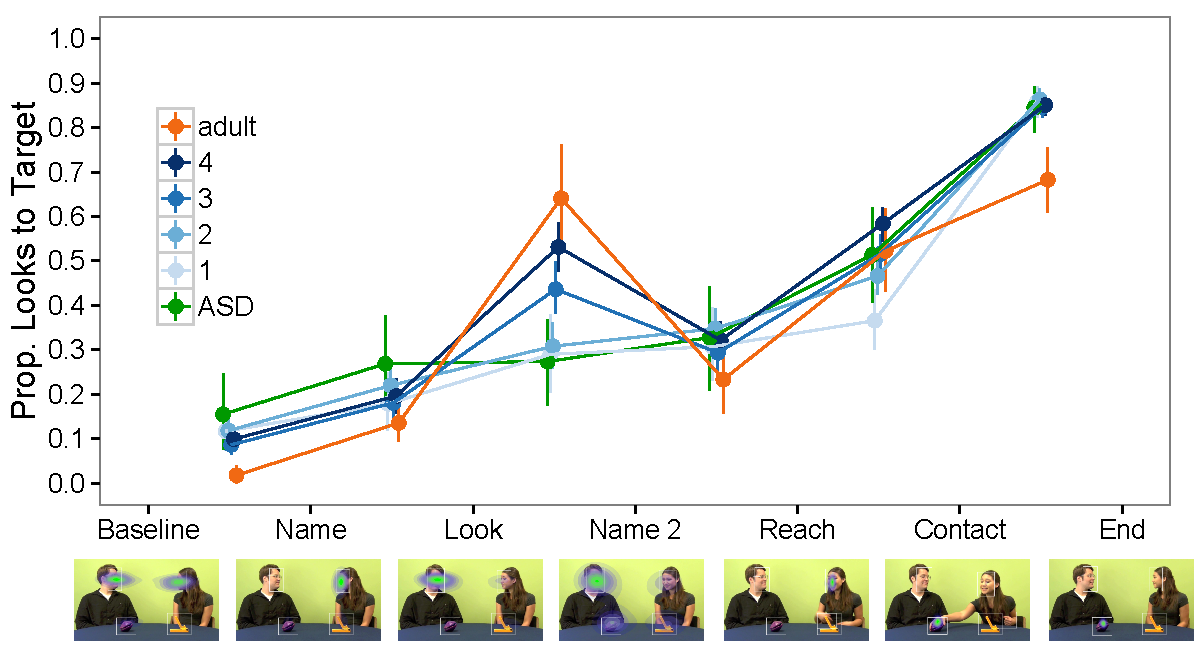
\includegraphics[width=.95\textwidth]{figures/bronto_all.pdf}
	\caption{\label{fig:reflook_learning} (bottom) Looking to target vs. competitor objects during the learning portion of Experiments 1 (typically-developing children) and 2 (ASD children), plotted by phase of the naming event. Points show means and error bars show 95\% confidence interval across participants; points are offset on the horizontal to avoid overplotting. (bottom) Example frames from the first word learning dialogue in Experiment 1. Each image shows the regions of interest used for later analysis (white boxes) and a heat map of the entire participant group's average point of gaze (hotter colors indicate more fixation; scale is constant across frames)}
\end{figure*}

In three experiments, we test the hypothesis that social attention allocation is a bottleneck in early word learning. We constructed videos that used novel words in a series of naturalistic object-focused dialogues and monologues. These videos were intended to be sufficiently difficult in their structure that in-the-moment disambiguation would pose a significant challenge to young learners, yet sufficiently simple that co-occurrence information could allow for successful word learning. We measured children's eye-movements during viewing as an index of their online inferences about the current conversational referent, and then tested their retention of the words they learned via a series of forced-choice test trials. These rich time-course data allowed us to test the hypothesis that those children who were successful in attending to the conversational referent would be the same children who learned and retained the words. 

In Experiment 1, we measure developmental changes in social information processing and use these to predict word learning in typically developing children. In Experiment 2, we tested a sample of children diagnosed with autism spectrum disorder in the same paradigm as Experiment 1 to determine if social attention was a bottleneck on their learning from these videos in the same way as for the typically developing children. In Experiment 3, we manipulate the timing of social information directly to test the causal role of fast social attention, again in typically developing children. In all three studies, we recruit children across a broad age range, giving us the power to see continuous changes in both social attention and novel word learning. 

\section{Experiment 1: Social Attention and Word Learning}

Experiment 1 was designed to estimate the developmental trajectory of children's online social information process in complex interactions, and to ask whether this processing had downstream consequences for word learning. The experiment consisted of two parts: learning and test. During the learning part, participants watched a series of dialogues and monologues in which actors introduced and discussed two novel objects and two familiar objects. Each video contained two naming sequences (pictured in Fig.~\ref{fig:reflook_learning}, bottom); these sequences were broken into a series of phases during which the speaker named, looked at, named again, and reached for a particular object, allowing for the separate measurement of name-, gaze-, and reaching-related changes of attention. 

We first measured the proportion of time participants spent looking at the target referent during the naming sequences in which the novel objects were introduced (Fig. ~\ref{fig:reflook_learning}). We analyzed these trajectories by fitting a mixed-effects model predicting looking at the target from naming phase, age, and their interaction. Children increased their looking to the correct over the course of learning trials, with above-baseline looks to the target in all phases after the second naming, with looking reaching nearly 100\% by the end of these events after the speaker had made contact with the toy ($\beta_{name2-reach} = .18$, $t = 3.73$, $p < .001$; $\beta_{reach_contact} = .13$, $t = 2.56$, $p < .01$; $\beta_{contact-end} = .75$, $t = 15.8$, $p < .001$). The effect of age was not significant, but there was a significant interaction---older children looked significantly more in the phases after the speaker's initial look and initial reach ($\beta_{look-name2} = .11$, $t = 7.66$, $p < .001$ ; $\beta_{reach-contact} = .08$, $t = 5.83$, $p < .001$). While the youngest children were only occasionally able to quickly follow the speaker's social cues, older children and adults were much more sensitive. Thus, the ability to quickly and reliably follow a speaker's social  online in a naturalistic conversation appears to develop significantly over the course of the first five years, and even further into adulthood.

Next, to measure children's retention of the novel words they were exposed to during the learning portion of the experiment, during the test trials we showed them pairs of toys and labeled one, using a standard looking-while-listening procedure \cite{fernald1998, fernald2008}. To measure online language comprehension more generally, we also included familiar word trials (Fig.~\ref{fig:reflook_test}. Children in all age groups successfully looked at familiar referents at above chance levels (smallest $\mu_{1-year} = .57$, $t(28) = 4.05$, $p < .001$), and all but the one-year-olds reliably learned the novel words (smallest $\mu_{2-year} = .56$, $t(53) = 3.89$, $p < .001$). A linear model showed that children performed better on test over development ($\beta_{age} = .07$, $z = 7.93$, $p < .001$), and that the effect of age was greater for familiar than novel trials ($\beta_{age * novel} = -.012$, $z = -2.42$, $p < .05$)

Thus, older children learned more from the same naming events. However, these children also improved on both other measures --- quickly following speaker's social cues gaze and reach, and processing familiar words. All of these factors were independently, significantly correlated with learning ($r_{age}(197) = .29$, $p < .001$); $r_{familiar}(197) = .20$, $p < .01$; $r_{look-name2}(192) = .34$, $p < .001$; $r_{reach-contact}(194) = .16$, $p < .05$). Which of these factors was most responsible for improvements in learning? To answer this question, we fit a linear regression, predicting learning on from age, familiar word processing, and looking to the target in the two relevant windows---after the look, and after the reach. Only looking to the target referent following the initial look reached significance ($\beta_{look-name2} = .14$, $z = 3.31$, $p < .01$), although age was marginal ($\beta_{age} = .02$, $z = 1.66$, $p = .1$). Because these predictors were all correlated, we also fit this same model after first residualizing out the effect of age on learning. In this model, gaze-following still remained highly significant ($\beta_{look-name2} = .12$, $z = 2.94$, $p < .01$).

Thus, age-related improvements in social attention, whatever their cause, are a critical bottleneck on learning from naming events throughout early childhood. Put another way, the age-related changes in word learning that we saw appeared to be accounted for largely by changes in social attention.

\section{Experiment 2: Social Attention in Autistic Children}

The naming events in Experiment 1 contained information sufficient to infer the meanings of the novel words at two timescales: (1) within the interactions, by following the informative social cues, and (2) across the interactions, by using co-occurrence statistics between the words and objects. While typically developing children's social information processing predicting a large chunk of the variance in their word learning, it is possible that atypically developing children would use a different strategy.

We tested a group of 38 children diagnosed with Autism Spectrum Disorder who, due to deficits in social information processing, might be expected to learn predominantly from the cross-situational statistics instead. These children did indeed process social information less efficiently---following the speaker's gaze no better than the youngest children in our sample (Fig.~\ref{fig:reflook_learning}. They also learned learned the Novel words, and attended to the referents of Familiar words at approximately the same levels (Fig.~\ref{fig:reflook_test}). However, while age was uncorrelated  word learning for the Autistic children ($r(25) = .14$, $p =.49$), following the speaker's gaze was highly correlated with Novel word learning ($r(20) = .58$, $p <.01$), just as in the typically developing sample. We again fit a linear regression, predicting learning on from age, familiar word processing, and looking to the target in the two relevant windows---after the look, and after the reach. This model showed significant effects of familiar word processing ($\beta_{familiar} = .54$, $z = 2.73$, $p < . 051$) and gaze following  ($\beta_{look-name2} = .23$, $z = 2.696$, $p < .01$).

Thus, social information processing remains a critical bottleneck on word learning in autistic children, just as in typically developing children.


\begin{figure}[tb]
	\center{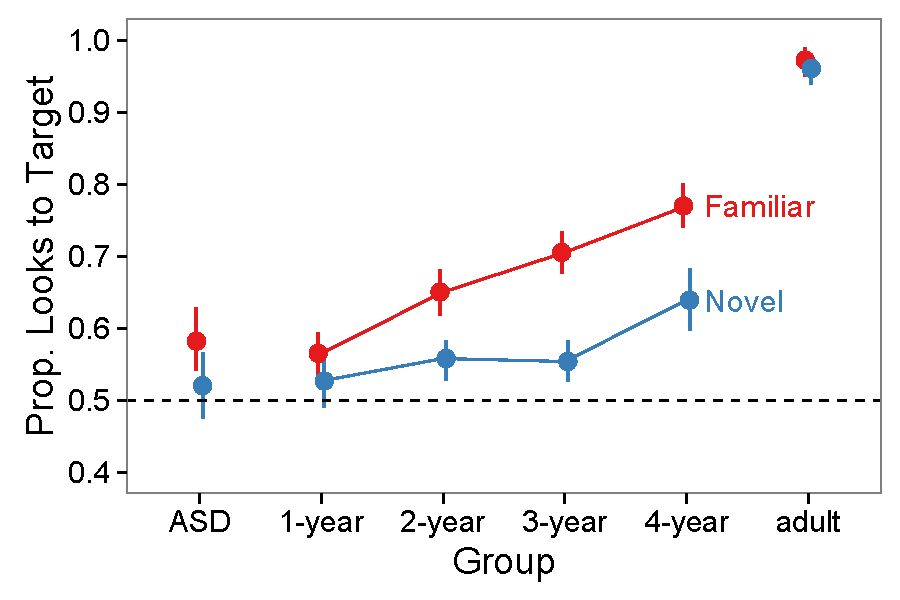
\includegraphics[width=.5\textwidth]{figures/reflook_test.pdf}}
	\caption{\label{fig:reflook_test} Test trial performance in for children and adults Experiment 1, as well children with ASD in Experiment 2. Colors show Familiar and Novel word trials, and error bars show 95\% confidence intervals computed by non-parametric bootstrap. Points are offset on the horizontal to avoid overplotting.}
\end{figure}

\section{Experiment 3: Varying Demands on Social Attention}

The naming events in Experiment 1 provided children with a number of informative cues to the referents of the novel words: social gaze, speaker's manual interaction, and also cross-situational co-occurrence statistics. Our analysis showed that fast processing of social gaze was the primary predictor of ultimate word learning. In Experiment 2, we tested this prediction directly. 

In Experiment 2, the two Novel words were introduced in two different kinds of naming events. In Extended Hold events, the speaker made contact with and manipulated the target toy for the duration of the naming event, providing an extended cue to the target of her referential intention. In contrast, on Brief Look trials, the speaker only provided punctate gaze information, looking to the target of her referential utterance briefly after naming it and then looking forward towards the camera for the remainder of the naming event. On the basis of the results from Experiments 1 and 2, we predicted that Extended Hold trials would show less developmental differentiation in social attention and be easier to learn from. In contrast, we predicted that following the Brief Look would require rapid reallocation of social attention, and thus that older children would succeed while younger children failed. Further, we predicted that this would produce down-stream differences in learning.

As predicted, on Extended Hold trials, children's spent a large proportion of the naming events looking at the target across age groups ($\mu_{1-year} = .57$, $\mu_{2-year} = .60$, $\mu_{3-year} = .63$, $\mu_{4-year} = .60$), and there was not a signfiicant correlation between age and looking ($r(290) = .08, p = .15$). In contrast, children spent a much lower proportion of Brief Look events looking at the target, and this proportion increased across age ($\mu_{1-year} = .09$, $\mu_{2-year} = .09$, $\mu_{3-year} = .16$, $\mu_{4-year} = .17$; $r(288) = .27$, $p  < .001$). 

As before children in all age groups showed evidence of processing familiar words at above chance levels (smallest $\mu_{1-year} = .59$, $t(63) = 5.09$, $p < .001$). Children 2-years-old and older showed evidence of learning from the Extended Hold trials (smallest $\mu_{2-year} = .63$, $t(66) = 5.43$, $p < .001$), and only the 3- and 4-year-olds learned from the Brief Look trials (smallest $\mu_{3-year} = .58$, $t(68) = 3.66$, $p < .001$). To confirm these analyses, we fit a mixed effects model predicting looking at test from age and trial type, finding significant effects of both ($\beta_{age} = .08$, $t = 19.34$, $p < . 001$; $\beta_{Familiar} = .09$, $t = 6.64$, $p < . 001$; $\beta_{Brief Look} = -.09$, $t = -6.48$, $p < . 001$).

To succeed on test trials, children needed to succeed on two tasks: 1. Process social information to disambiguate naming events and discover the speaker's intended referent, and 2. Recall the learned mapping and use it to find the correct referent. The two kinds of naming events in this experiment were designed to vary in how much demand they placed on (1), but not on (2). To provide an additional test of our prediction, we fit a mixed effects model predicting children's looking on Novel test trials from their age, their Familiar word processing, and the naming event type, as well as the interaction of familiar processing and test type. This model showed a significant effect of age ($\beta_{age} = .05$, $t = 4.83$, $p < . 001$), as well as a significant interaction between Familiar word processing and naming event type($\beta_{Extended Hold * Familiar} = .21$, $t = 3.47$, $p < . 001$). That is, Familiar word processing was a better predictor of children's success on Extended Hold trials, where it was the primary bottleneck. 

%Intriguingly, the difference between Extended Hold and Brief Look appeared to vary across across development. For 1-year-olds who did not appear to learn from the Extended Hold, it is perhaps unsurprising that they also learned little from the Brief Look. However, the difference between the Brief Look and Extended Hold appeared to be attenuated for the 4-year-olds relative to the 2- and 2-year olds. 

Together, these results demonstrate the powerful role of fast social information processing in early word learning. All of the children were able to follow the speaker's social cues when they extended over the entire naming event, and this supported their learning. In contrast, only the older children were able to follow the brief look, and only they were consequently able to learn from it. 


\begin{figure}[h]
	\center{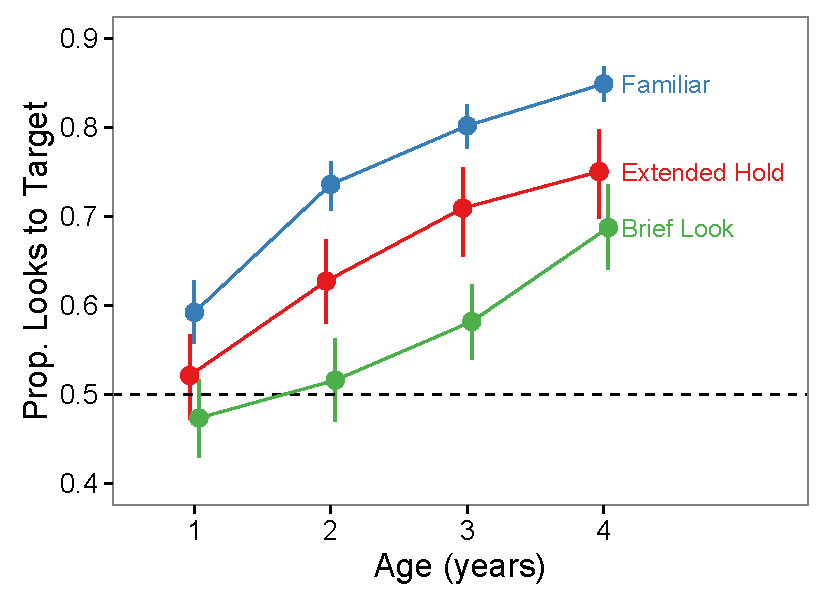
\includegraphics[width=.5\textwidth]{figures/soc_word_test.pdf}}
	\caption{\label{fig:soc_word_test} Test trial performance in Experiment 3 for the Familiar words, as well as for Novel words that appeared in Brief Look and in Extended Hold learning events. Error bars show 95\% confidence intervals computed by non-parametric bootstrap; points are offset on the horizontal to avoid overplotting.}
\end{figure}

\section{Discussion}

\begin{materials}

\subsection{Participants} Data from typically-developing children was collected at the San Jose Children's Discovery Museum, where parents and their children were invited to participate in an experiment investigating children's early word learning. In Experiment 1, we collected both demographic and eye-tracking data from 349 children in the target age range, of whom 113 were excluded from the final sample for one or more of the following reasons: unacceptable eye-tracker calibration or data ($N=52$), atypical development developmental trajectories ($N=30$), and less than 75\% parent-reported exposure to English ($N=40$). Our final sample included 236 children (41 1-year-olds (21 girls); 66 2-year-olds (32 girls); 73 3-year-olds (36 girls); and 56 4-year-olds (30 girls)). In Experiment 2, we collected demographic and eye-tracking data from 425 children in the target age range, of whom 201 were excluded from the final sample for one or more of the following reasons: unacceptable eye-tracker calibration or data ($N=96$), atypical development developmental trajectories ($N=36$), and less than 75\% parent-reported exposure to English ($N=48$). Our final sample included 224 children, ages 1 -- 5 (60 1-year-olds (24 girls); 57 2-year-olds (29 girls); 51 3-year-olds (25 girls); and 50 4-year-olds (24 girls)).

Data from Autistic children was collected at Stanford University, where parents and their children.... We demographic and eye-tracking data from 47 1--7-year old-children, of whom 11 were excluded for unacceptable eye-tracker calibration. The final sample comprised 38 children ($M_{age}$ = 4.28-years, range = (2.24--7.97-years), 4 girls). Adult participants in Experiment 1 were 17 Stanford undergraduate students who participated in exchange for course credit.

\subsection{Stimulus and Design} After an initial eye-tracker calibration phase, children and adults in both experiments watched a $\sim$6 minute video. Each video presented two kinds of trials. Learning trials consisted of videos in which speakers seated at a table with two toys provided social cues and labelled one of the toys. Test trials showed pictures of two objects on a black background while a voice asked the participant to look at one of them \cite[as in][]{fernald1998}. 

In addition, each video included a re-calibration stimulus which participants saw a small, brightly colored stimulus move around the screen. These phases of the videos were used to correct the calibrations estimated at the beginning of the experiment \cite[see][]{frank2012}. Finally, videos contained a small number of filler trials in which participants saw engaging pictures or videos designed to keep maintain their attention for the duration of the video.

Learning trials varied across the Experiments. In Experiment 1 and 2, these learning trials consisted of two dialogues in which two speakers sat at a table together, and one referred to teach of the two novel toys whose names were taught in the experiment (``toma'' and ``fep''). The other two learning trials were monologues in which one of the speakers sat at a table alone, with one of the novel toys and one familiar toy and referred to each in turn. Each naming event consisted of six events: first a naming phrase, the a look at the object accompanied by a comment, a second naming, a reach for the object, and finally a demonstration of the object's function accompanied by a third naming. Each novel object was named nine times in total over the course of the video. Participants watched all of the learning trials before they began the test trials. Eight of these test trials tested familiar objects (e.g. dog/car or lamp/carrot); the other eight paired the two novel objects. Naming phrases were of the form ``Look at the [car/fep]! Do you see it?'' and were spoken by the actors in the video.


In Experiment 3, we simplified the learning trials. All naming sequences were monologues and both toys on the table were novel.  Four of the naming sequences these were Extended Hold trials, in which the speaker reached for and interacted with one of the two toys while describing its function and producing its name three times. The other four were Brief Look trials in which the speaker produced the same kind of description but indicated the target toy only with a brief look after first producing it's label. Brief Look and Extended Hold trials used a distinct but consistent set of two toys, and the same toy was consistently either the target or the competitor on each trial type. Because children in Experiment 1 sometimes lost interest in these videos before reaching the test trials, in Experiment 3 test trials were interspersed with learning trials so that at least some test data could be acquired from each child. In total, Experiment 3 contained 20 test trials. Eight of these test familiar objects as in Experiment 1s and 2. Eight paired the named objects from the learning trials against their foils from the learning trials, four each for the object named in Brief Look trials, and four for the object named in Extended Hold trials. The remaining four test trials paired the two named objects against each other, with children being asked to find each two times.

\subsection{Data Analysis}

In all experiments, raw gaze data went through several transformations before statistical tests were computed. First to ensure appropriate precision in region-of-interest analyses, infants' calibrations were corrected and verified via robust regression \cite[described in][]{frank2012}, and calibration corrections were assessed by two independent coders ($\kappa = FIXME$). Children whose calibrations could not be verified and corrected were excluded from further analyses.

Second, all analyses were performed use an Area of Interest (AOI) approach. On learning trials, AOIs were hand-coded frame-by-frame for each of the speakers' faces and for the two on-screen objects. On test trials, these AOIs corresponded to the static on-screen positions of the two alternatives. To use standard statistical analyses, we transformed the timecourse data to proportions of looking within relevant windows. On test trials the start of this window was set to 500ms after the point of disambiguation---the onset of the target label. The end of the window was set to the length of the shortest test trial for accurate averaging. This was 4s for Experiment 1, and 4.5s for Experiment 2. These windows were chosen to give all children sufficient time to process the label, and to maximize signal.

In Experiments 1 and 2, learning trials contained six distinct phases (Fig.~\ref{fig:reflook_learning}): a baseline period of exactly 2 s, name 1 to look (M = 1.7 s), look to name 2 (M = 2.0 s), name 2 to initiation of reach (M= 4.8 s), initiation of reach to point of contact (M = .8 s), and after contact with the object (M = 1 s). Proportion of looks to the target AOI were computed in each of these windows. In Experiment 2, learning trials were designed to separate demands on social attention across rather than within trials. In Experiment 2, we computed proportion of looking of the entirety of learning trials.

Due to occasional bouts of inattention, eye-gaze data was not available for all children during all portions of the experiment. To correct for statistical errors introduced by averaging over small windows,
data from individual learning and test trials was excluded from analysis if less than 50\% of the window contained eye-tracking data (regardless of where children were looking). Second, if more than 50\% of the trials a given participant were excluded in this manner, all of the remaining trials were dropped as well. All data and analysis code are freely available at a public GitHub repository at \small{\tt{http://github.com/dyurovsky/refword}}.

\end{materials}

\begin{acknowledgments}
We gratefully acknowledge the parents and children who participated in this research and the staff of the San Jose Children's Discovery Museum for their collaboration on this line of research. This work was supported by NIH NRSA F32HD075577 to DY,  and grants from the John Merck Scholars program, the Stanford Child Health Research Initiative to MCF .
\end{acknowledgments}

\bibliographystyle{pnas2011}
\bibliography{refword}

\end{article}

\end{document}
